\section{Belief-State JEPA}
\label{sec:architecture}

\begin{figure*}[t]
  \centering
  \begin{subfigure}[b]{0.48\textwidth}
    \centering
    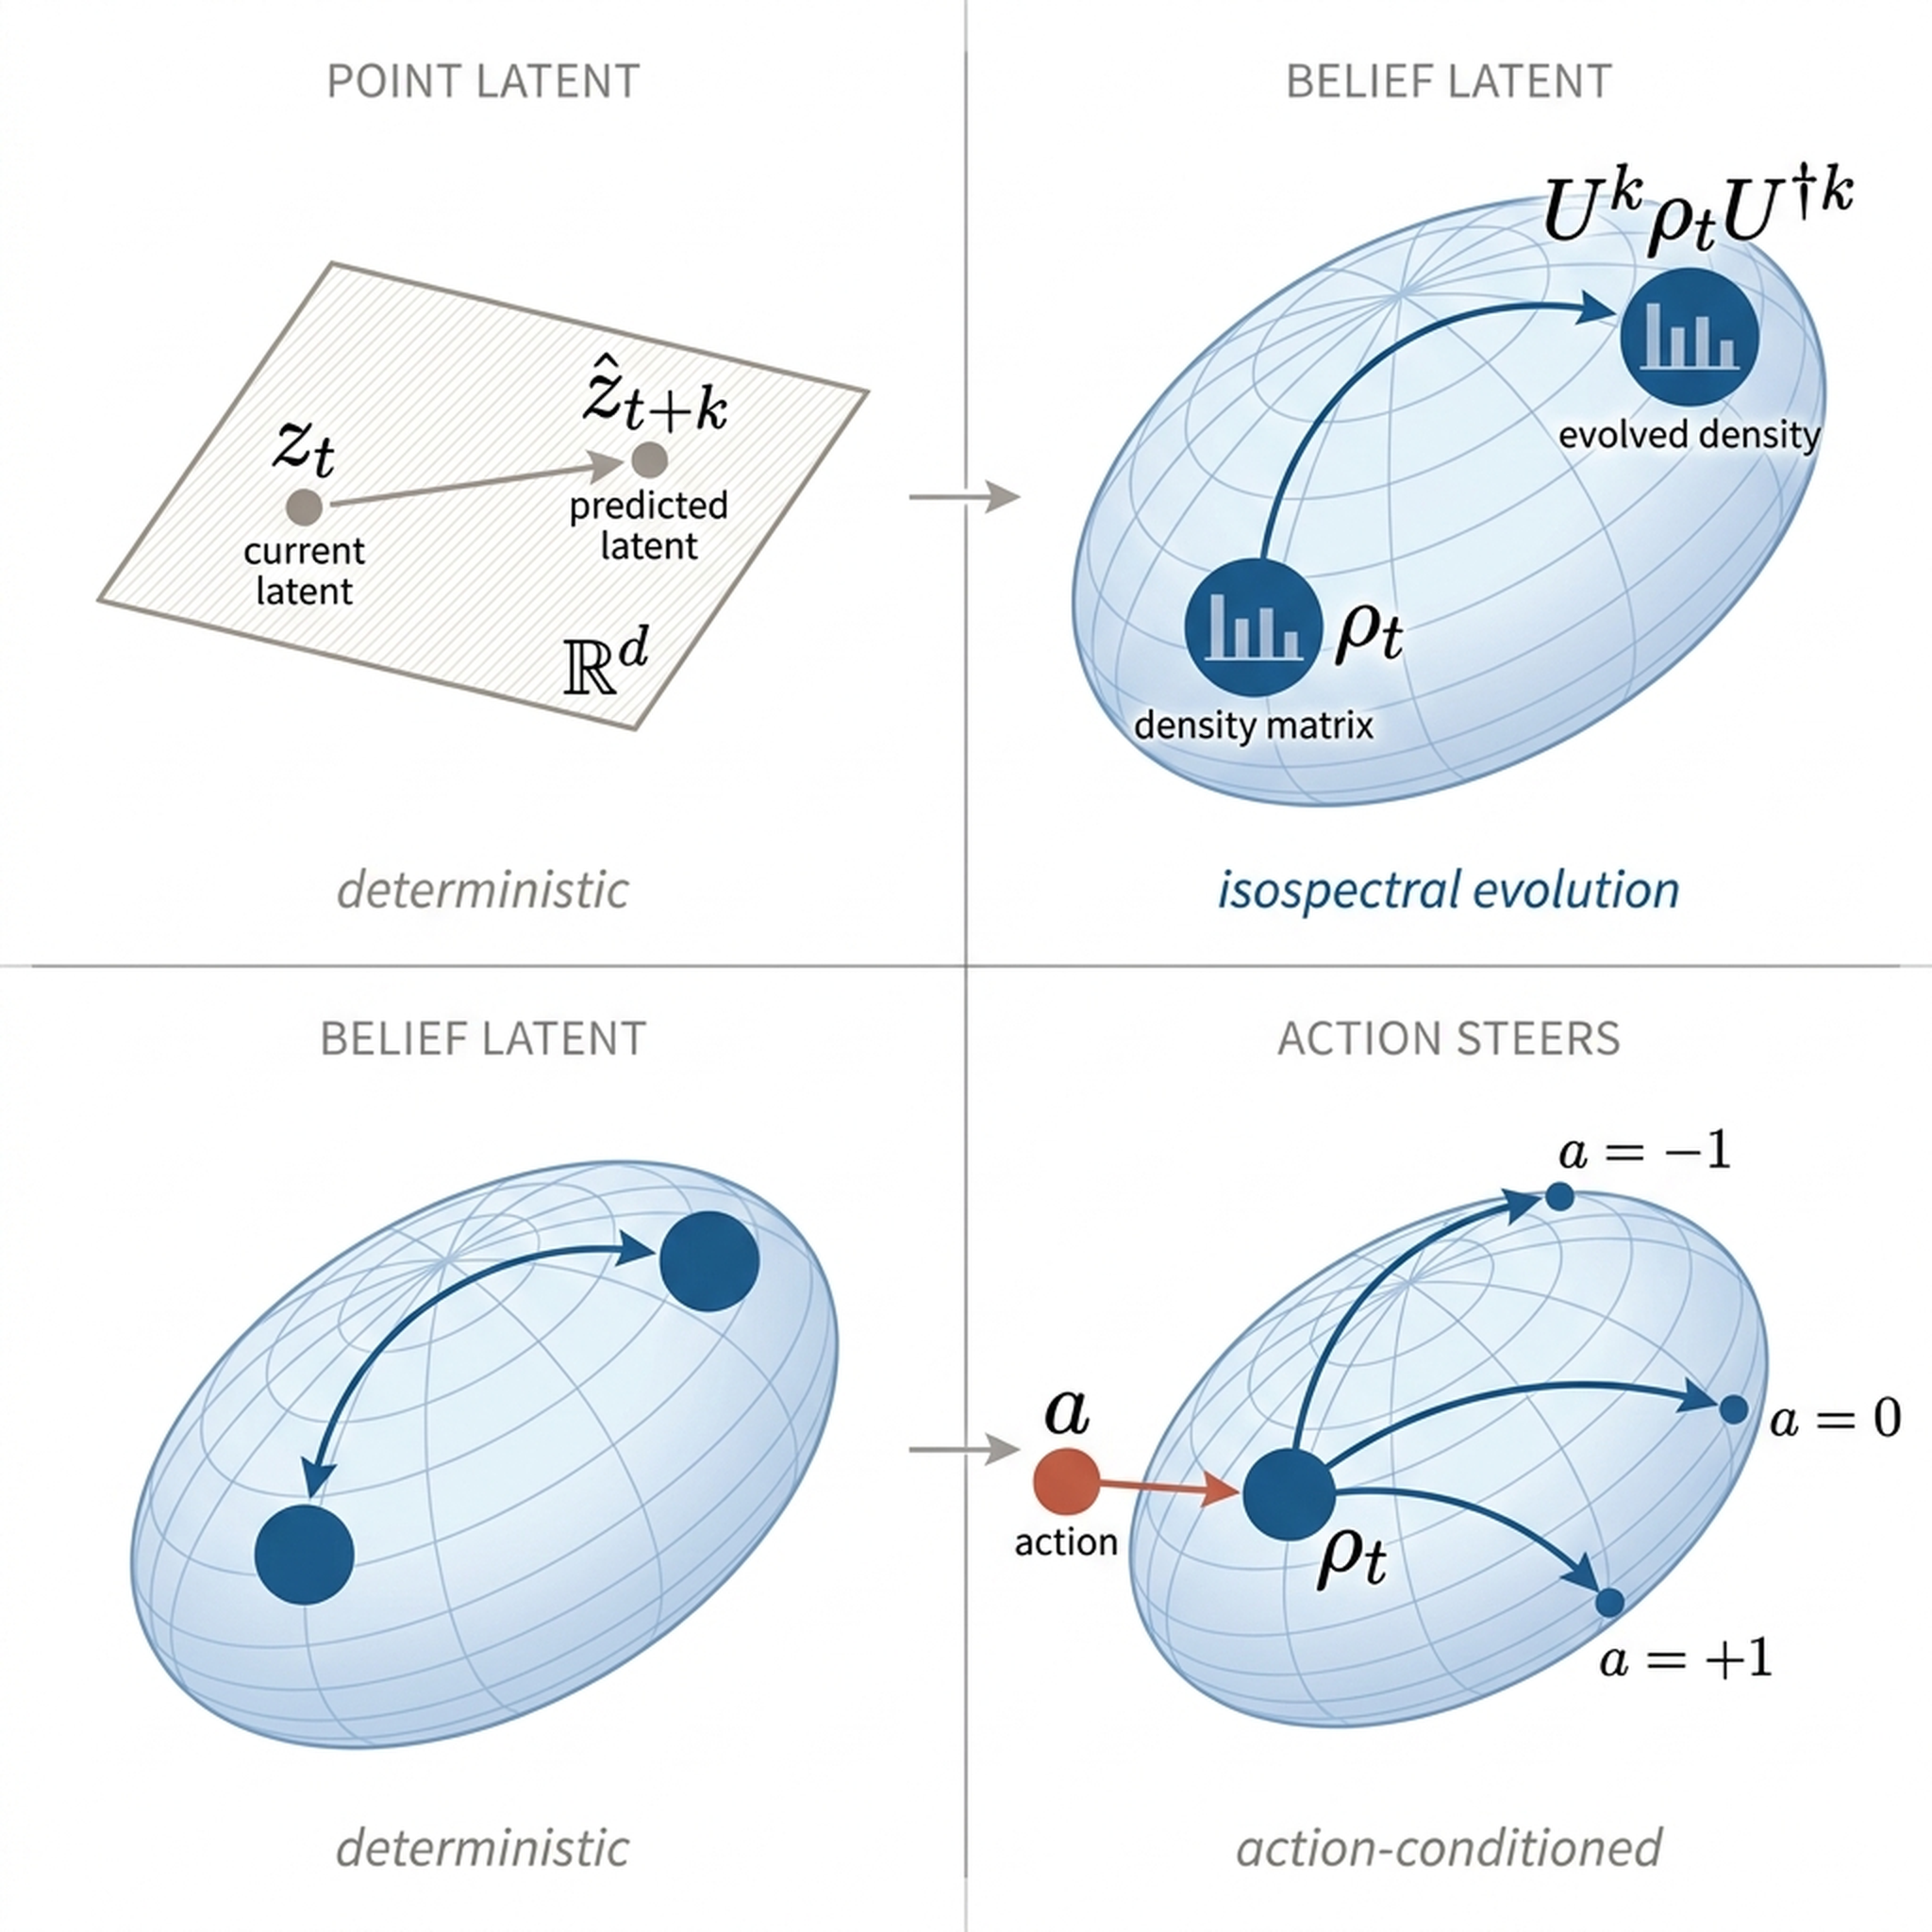
\includegraphics[width=\linewidth]{figures/fig_hero.png}
    \caption{Concept: point vs.\ belief latent.}
    \label{fig:hero}
  \end{subfigure}
  \hfill
  \begin{subfigure}[b]{0.48\textwidth}
    \centering
    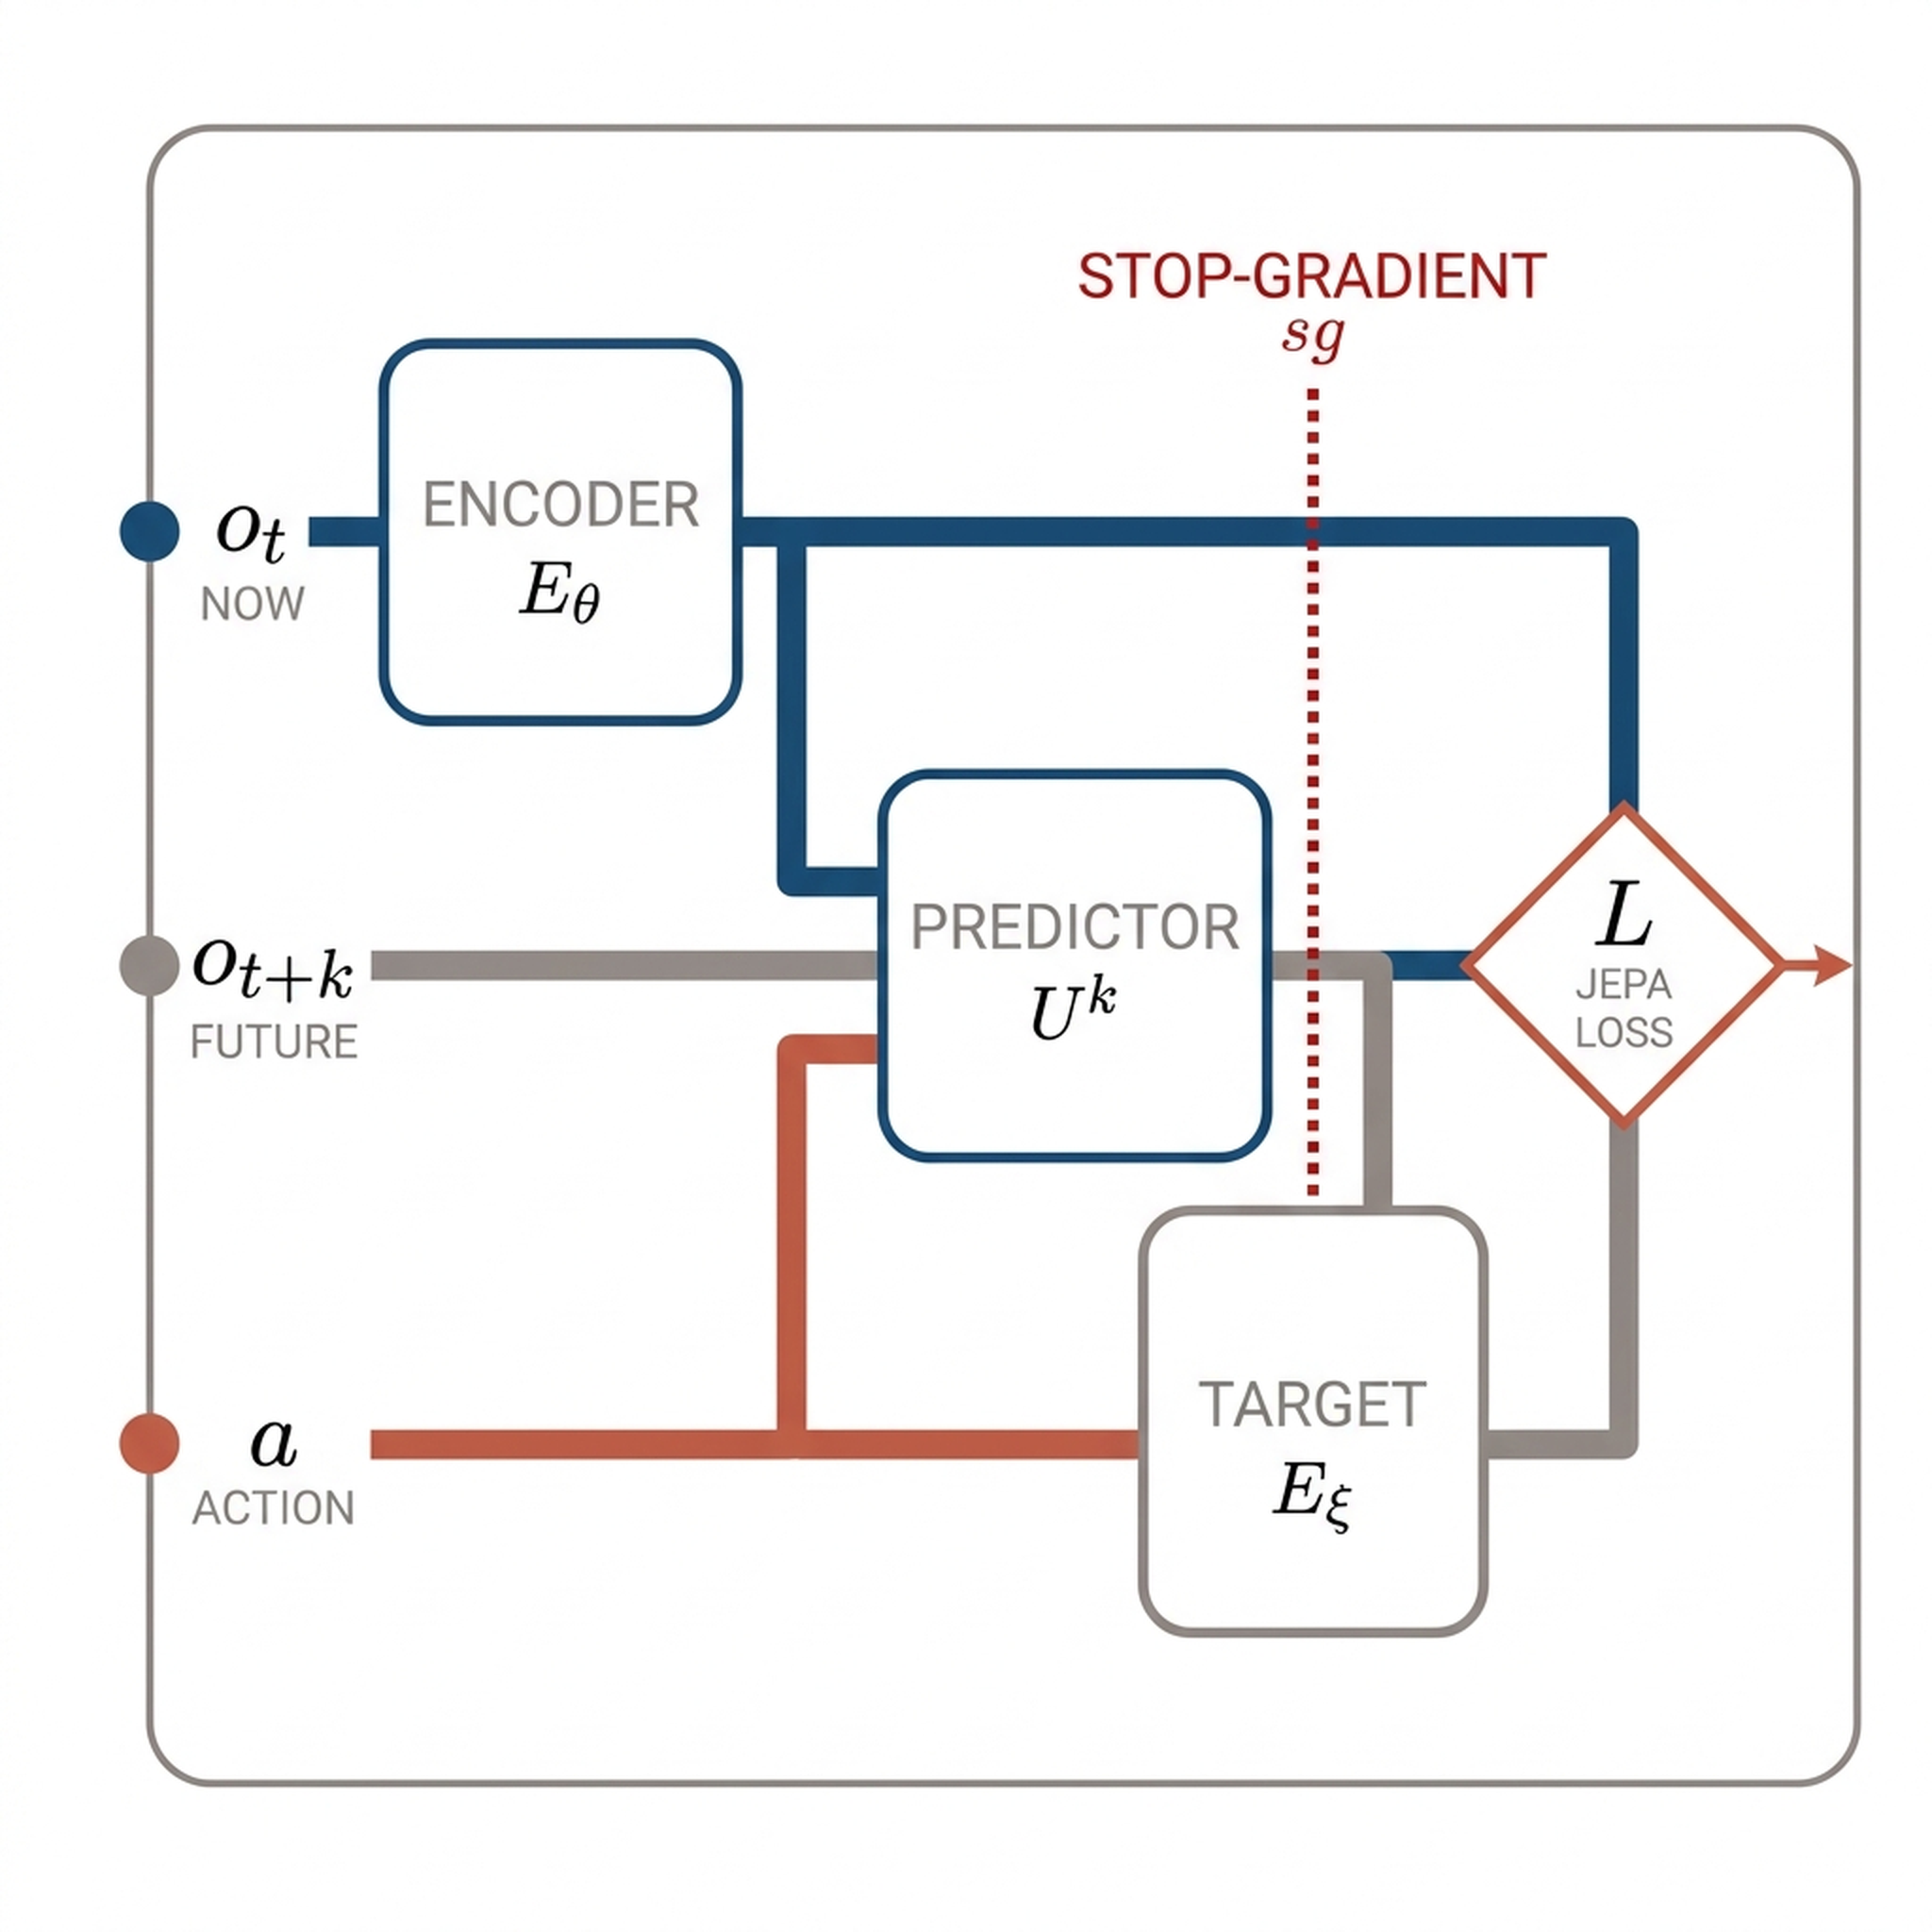
\includegraphics[width=\linewidth]{figures/fig_architecture.png}
    \caption{Architecture: JEPA scaffold with unitary predictor.}
    \label{fig:architecture}
  \end{subfigure}
  \caption{\textbf{From point latents to belief-structured imagination,
  and the architecture that realises it.}
  \textbf{(\subref{fig:hero})} A standard vector-latent JEPA predicts a
  point in representation space. UWM-JEPA instead represents the latent
  as a density matrix and rolls it forward on an isospectral orbit.
  Under partial observability this gives the predictor a structured
  latent in which uncertainty and hidden modes can be carried through
  blind rollout; actions steer the unitary trajectory through
  $H(a)=H_0+aH_1$.
  \textbf{(\subref{fig:architecture})} The online encoder maps the
  current observation history to $\rho_t$; the predictor applies
  $U^k\rho_t(U^\dagger)^k$ or an action-conditioned sequence
  $U(a_{t+k-1})\cdots U(a_t)\rho_t U(a_t)^\dagger\cdots U(a_{t+k-1})^\dagger$.
  The EMA target encoder supplies the stop-gradient future target, and
  the JEPA loss is evaluated after the system readout and projection.}
  \label{fig:overview}
\end{figure*}

UWM-JEPA modifies the \emph{predictor} of a JEPA-family world model
and leaves the surrounding training protocol unchanged. Given a
partially observed sequence $o_{\le t}$, the online encoder
$E_\theta$ produces a joint density matrix
\begin{equation}
  \rho_t \in \mathbb{C}^{\dtot \times \dtot},
  \qquad
  \rho_t=\rho_t^\dagger,\quad
  \rho_t\succeq 0,\quad
  \Tr(\rho_t)=1,
  \label{eq:density-latent}
\end{equation}
on a bipartite latent space
$\mathcal{H}_{\tot}=\mathcal{H}_{\sys}\otimes\mathcal{H}_{\env}$~\cite{nielsen2010quantum,breuer2002theory}.
All experiments use $\dsys=8$, $\denv=2$, and $\dtot=16$. The system
factor is the part read by the JEPA loss and by downstream probes; the
environment factor gives the model a register in which hidden modes
and system--environment correlations can be carried during rollout.
The practical readout is the reduced state
$\rho_t^{\sys}=\Tr_{\env}\rho_t$~\cite{nielsen2010quantum}.

The density-matrix constraints are enforced by construction. The
initial state is maximally mixed on the joint space; each observation
update sandwiches the current state by a positive system measurement
operator lifted as $K(o_t)\otimes I_{\env}$ and then renormalises to
unit trace; each prediction step is unitary conjugation. These
operations preserve Hermiticity and positive semidefiniteness up to
numerical symmetrisation, so the conditions in
\cref{eq:density-latent} are an invariant of the recurrence rather
than an unconstrained decoder output.

The prediction operator is the central architectural choice. For a
horizon $k$, UWM-JEPA rolls the latent forward by unitary conjugation,
\begin{equation}
  P_k(\rho_t)=U^k\rho_t(U^\dagger)^k,
  \qquad
  U=\exp(-iH\Delta t),\quad H=H^\dagger.
  \label{eq:predictor}
\end{equation}
Blind rollout therefore traces the unitary orbit of the joint density
matrix rather than an unconstrained vector trajectory. The target
branch follows the usual JEPA construction: an EMA encoder $E_\xi$
produces $\tilde\rho_{t+k}=E_\xi(o_{\le t+k})$ with stop-gradient on
the target parameters~\cite{grill2020bootstrap,tarvainen2017mean,caron2021emerging,chen2021exploring},
\begin{equation}
  \xi \leftarrow \tau \xi + (1-\tau)\theta,
  \qquad
  \nabla_\xi \mathcal{L}_{\mathrm{JEPA}}=0.
  \label{eq:ema-target}
\end{equation}
The loss is evaluated after reduction to the system factor and after a
small projection head $g_\phi$. Writing
$\hat h_{t+k}=g_\phi(\Tr_{\env}P_k(E_\theta(o_{\le t})))$ and
$h^+_{t+k}=g_\phi(\Tr_{\env}E_\xi(o_{\le t+k}))$, the objective is
\begin{equation}
  \mathcal{L}_{\mathrm{JEPA}}
  =
  \left\|
  \hat h_{t+k}-\mathrm{sg}\!\left[h^+_{t+k}\right]
  \right\|_F^2 .
  \label{eq:jepa-loss}
\end{equation}
The model therefore exposes two readouts. The structural guarantee
in the next section is exact on the \emph{joint} state, while the
learned objective and all downstream probes operate after partial
trace and projection.

Actions enter through an action-conditioned generator,
$H(a)=H_0+aH_1$~\cite{horowitz2022quantum,greydanus2019hamiltonian},
with rollout governed by the corresponding sequence of unitaries. The
action experiments below compare teacher-forced and counterfactual
\emph{targets} while holding the JEPA scaffold fixed, isolating the
target-construction effect from architectural changes to the predictor.
